\newpage
\chapter{Design Error Analysis}\label{designerror}

    %In this chapter, the focus is on situations where a designed E/E architecture is not satisfiable meaning feasible solutions are not found by the solver. In contrast to simple models, navigating and correcting unsatisfiability of complex E/E models is an elaborate and time-consuming task, and increases the development costs.
    
    This chapter focuses on situations where a designed E/E architecture is not satisfiable, which means that the solver cannot find feasible solutions. Unlike simple models, navigating and correcting the unsatisfiability of complex E/E models is an intricate and time-consuming task, leading to increased development costs.
    
    %To tackle this problem, an approach is introduced to identify design errors in case of having violations in the constraint setincluded in the system model after solving step. This feature is important for identifyingand addressing errors in the system design with a reasonable amount of time, ensuringthat the system is optimized and meets all necessary constraints and requirements.
    To address this issue, an approach is introduced to identify design errors when violations occur in the constraint set included in the system model after the solving step. This feature is crucial for detecting and rectifying errors in the system design within a reasonable timeframe, ensuring that the system is optimized and meets all necessary constraints and requirements~\cite{askaripoor2023designer,askaripoor2022architecture,9613692}.
    
    %To tackle this problem, a constraint labeling approach is presented which aims to assist the designers to better understand where in the model the unsatisfiability occurs i. e. there are conflicting constraints that cannot be satisfied at the same time. 
    
    %Only if the solving procedure terminates within acceptable time (depending on engineering requirements), network configuration or model correction can be started. To optimize the model before synthesis, Prolog-based queries are presented which aim at reducing the synthesis time by optimizing the network model. 
    \section{Background}
    
    %In many fields of technology and science, a common approach to solvingproblems involves finding solutions that satisfy a set of formal constraints. These constraint systems are employed in a range of areas, including formal verification and automated configuration of hardware or software, planning problems, and other applications of artificial intelligence.Propositional logic is one of the most widely used formalisms for representing constraints. It enables to model logical relations between facts that are either true or false. The satisfiability (SAT) problem is concerned with determining if there exists a combination of facts for which a propositional formula holds. Due to its NP-completeness, the SAT problem is essential in many areas of computer science, and no known algorithm can solve every instance efficiently. A significant area of research in formal methods focuses on unsatisfiable constraint sets, where sets of constraints are shown to be unsatisfiable by formal means. In many applications, such sets arise from design errors that we aim to detect. An effective way to gain insights into such errors is to extract from a set of conflicting constraints a minimal explanation that clarifies which constraints or interactions between constraints are problematic. 
    
    In numerous domains of technology and science, a prevalent problem-solving strategy involves discovering solutions that meet a set of formal constraints. These constraint systems are utilized across various sectors, including formal verification, automated configuration of hardware or software, planning tasks, and other applications within artificial intelligence.
    
    Propositional logic stands out as an extensively used formal framework for representing constraints. It facilitates modeling logical connections between facts that can be either true or false~\cite{buning1999propositional}. The boolean satisfiability (SAT) problem concerns determining whether a combination of facts makes a propositional formula valid. Due to its NP-completeness, the SAT problem plays a crucial role in many realms of computer science, and there's no known algorithm capable of efficiently solving every instance~\cite{biere2009handbook}. A substantial area of formal methods research focuses on unsatisfiable constraint sets where sets of constraints are proven unsolvable through formal methodologies. In various scenarios, such sets emerge due to design flaws it aims to identify. A productive approach to gaining insights into these errors involves extracting a minimal explanation from a collection of conflicting constraints. This explanation elucidates which constraints or interactions between them are causing the issue. 
    
    In the context of the SAT problem, constraints are expressed using formulas in propositional logic. In this scenario, every variable has a binary value of either TRUE or FALSE. When the constraint conditions are met, the outcome of the boolean logic evaluation is considered True. Conversely, if the conditions are unmet, the result is False~\cite{biere2009handbook}. Conventionally, SAT problems are often represented using conjunctive normal form (CNF)~\cite{sulflow2008using}.
    
    %Typically, conjunctive normal form (CNF) is used to represent SAT problems~\cite{sulflow2008using}.
    
    %One practical example of an unsatisfiable constraint system is found in automotive control systems for autonomous driving. These systems must incorporate safety-critical applications, software components, and hardware. When requirements for the safety-critical application, software, or hardware conflict, the result is an unsatisfiable constraint system. As autonomous driving technology advances, the complexity and functionality of automotive control systems, such as Driving Assistance Systems (ADAS) and Automated Driving Systems (ADS), increases, making it increasingly difficult to identify the minimal unsatisfiable core responsible for unsatisfiability in ADS. 
    
    %While most current research focuses on how to extract minimal unsatisfiable sets in an unsatisfiable constraint system, few studies explore how to identify the requirements and correct them to make the constraint system satisfiable.
    %Therefore, this chapter aims to address this gap by exploring the process of identifying minimal unsatisfiable sets related to the introduced set of constraints in the framework, and proposing practical solutionsto make the constraints satisfiable.
    
    Although most of present research is directed towards extracting minimal unsatisfiable sets from an unsatisfiable constraint system, only a few studies delve into recognizing requirements and rectifying them to transform the constraint system into a satisfiable state.
    Hence, this chapter aims to bridge this gap by investigating the process of identifying minimal unsatisfiable sets linked to the introduced set of constraints within the framework. In addition, this chapter suggests pragmatic approaches to render the constraints feasible.
    
    %The constraint system can be expressed in different ways depends on thedomain of its variables and the form of its constraints. Following someof the most commonly used formula and some important terminologies will be introduced.
   
    
    \subsection{Conjunctive Normal Form}
    
    CNF is a fundamental concept in propositional logic, a branch of formal logic that deals with manipulating and analyzing logical statements involving propositions and their truth values~\cite{sulflow2008using}. CNF serves as a structured representation for logical formulas, allowing complex statements to be broken down into simpler components that are easier to analyze, manipulate, and process using automated tools and algorithms.
    
    
    A logical formula is said to be in CNF if it is a conjunction $\wedge$ ($AND$) of one or more clauses, where each clause is a disjunction $\vee$ ($OR$) of literals. A literal is either a propositional variable (denoted by a letter or its negation) or the negation of a propositional variable. In CNF, the logical operators are reduced to only conjunction and disjunction.
    The following is a breakdown of the components of CNF:
    
    \begin{itemize}
        
        \item Clause: A clause is a disjunction of literals. It represents a statement that is true if at least one of the literals in the clause is true. For example, ($A$ $OR$ $B$) is a clause where $A$ and $B$ are literals. 
        
        \item Literal: A literal is either a propositional variable or the negation of a propositional variable. For example, $A$ and $\neg B$ (not $B$) are literals.
        
        \item Conjunction ($AND$/$\wedge$): The conjunction operator combines multiple clauses or literals with the $AND$ operator. It indicates that all the statements it connects must be valid for the entire formula to be true.
        
        \item Disjunction ($OR$/$\vee$): The disjunction operator combines literals within a clause. It indicates that at least one of the literals in the clause must be valid to be true.
    
    \end{itemize}
    %Putting it all together, here's an example of a logical formula in CNF:
    Below are examples of two formulas in CNF:

        \begin{equation}
            (A \vee \neg B) \wedge (\neg A \vee C) \wedge (B \vee C \vee D)
            \label{eq61}
        \end{equation}
        
            \begin{equation}
            (m_1 + m_2 \leq 3) \wedge (m_1 \geq 5) \wedge ( m_2 \leq 7) \wedge ( m_1 \leq 4).
            \label{eq62}
        \end{equation}\newline
        
    A CNF formula is satisfied when an assignment of truth values (true or false) to the variables in the formula makes the entire formula accurate. In other words, for a CNF formula to be satisfied, every clause within the formula must have at least one literal that evaluates to true under the given assignment. For example, the logical formula presented in~\eqref{eq61} consists of three clauses. To identify each clause, they are separated by $AND$/conjunctions. To determine if the CNF formula is satisfiable, it is required to find assignments for the variables ($A$, $B$, and $C$) that satisfy at least one literal in each clause. If $A$, $B$, $C$, and $D$ are set as TRUE, FALSE, FALSE, and TRUE, respectively, this assignment satisfies all clauses, so the CNF formula is satisfiable.
    
    Mathematical statement in \eqref{eq62} illustrates a CNF formula as a SMT interpretation including four clauses. Because of the conflicting $m_1$ clauses which define $m_1$ value, the CNF formula is unsatisfiable. 
    
    
    \subsection{Minimal Unsatisfiable Subset (MUS) or Unsatisfiable Core}
    %This task is effectively solved in practice, and the primary focus of this section centers around the most popular methods and techniques used to accomplish this.
    
    An unsatisfiable core, also known as a minimal unsatisfiable subset (MUS), is a subset of the original set of clauses (constraints) that, when taken together, is itself unsatisfiable. In other words, if any clause gets removed from the unsatisfiable core, the remaining subset becomes satisfiable.
    The concept of an unsatisfiable core is often utilized in solving constraint satisfaction problems, including SAT problems. It helps identify a smaller subset of conflicting clauses that are causing the unsatisfiability of the entire problem~\cite{sulflow2008using,biere2009handbook}.

    In the example presented in~\eqref{eq61}, the CNF clause, $B$ $\vee$ $C$ $\vee$ $D$, is considered. If $B$ and $C$ are both FALSE and $A$ is TRUE, the entire clause evaluates to TRUE, which means the original CNF formula is satisfiable.
    However, when dealing with a more extensive set of clauses and a particular combination of them results in an unsatisfiable formula, the goal is to identify the smallest possible subset of clauses responsible for the unsatisfiability. This subset is known as the unsatisfiable core.
    
    The concept of a MUS gives rise to various algorithmic tasks, showcasing significant differences in complexity and achievable performance and the methods employed to address them. Among these tasks, the simplest one entails discovering a single MUS, a process commonly called MUS extraction. Note that a minimal unsatisfiable subset may not necessarily be the smallest size, as smaller unsatisfiable subsets can exist. This simplifies the task into a linear search space traversal, continuing until a subset that fulfills the definition is found. 

    Moving to a more challenging endeavor, the aim is to uncover a MUS with the smallest possible cardinality, often known as the smallest MUS (SMUS). In other words, an SMUS is the most minor collection of constraints that cannot be satisfied simultaneously.
    In the realm of algorithms for this task, the initial reliance was on non-chronological backtracking~\cite{lynce2004computing}, although a more efficient approach has emerged in the form of a branch-and-bound technique~\cite{mneimneh2005branch}. However, the practical applicability of this problem appears to be somewhat limited. This is due to the fact that discovering a MUS of minimal size is notably more intricate than finding any MUS and frequently yields minimal additional information.
    The most ambitious task is exhaustively enumerating all MUSes within an unsatisfiable clause set. Current methodologies addressing this challenge incorporate ingenious enumeration techniques to optimize the assessment of subset candidates~\cite{de2003finding}. Alternatively, these methodologies capitalize on the duality shared by MUSes and maximal satisfiable subsets through an interleaved approach~\cite{bailey2005discovery} or a two-level approach~\cite{liffiton2008algorithms} to address a hypergraph transversal problem. Considering that a clause set may potentially comprise an exponential multitude of distinct MUSes, a universally efficient technique for identifying all MUSes is improbable. Nonetheless, even in substantial industrial scenarios, the count of unique MUSes often proves surprisingly limited, lending practical significance to extant tools for MUS enumeration. This significance arises from the collective set of MUSes offers an all-encompassing understanding of the underlying error's characteristics.
    
    %The SAT problem involves determining whether there exists an assignment of truth values that satisfies a given CNF formula. This problem has important applications in various areas, including artificial intelligence, formal verification, hardware and software design, and more. Tools and algorithms that solve the satisfiability problem are used to analyze the logical properties of systems, verify correctness conditions, and find solutions to a wide range of computational problems.
    
    
    
    
    %which shows as followed:
    %At its core, CNF provides a systematic way to express logical formulas as a conjunction (AND) of clauses, where each clause is a disjunction (OR) of literals. This format has widespread applications in various fields of computer science, including artificial intelligence, formal verification, logic programming, and automated theorem proving.
    
    \section{Approach}

    %The design error analysis approach aims at addressing the gap inidentifying the exact constraints that lead to model infeasibility in a constraintsystem. While previous studies focus on generating sets of    unsatisfiable or infeasible sets of constraints, the exact constraints thatcause the system to be infeasible are not thoroughly explored. This is important in the context of this thesis as finding the violated constraints after solving an extensive modeled E/E systems is extremely time-consuming and complex.Therefore, an approach is introduced to identify the core satisfiable constraint bybuilding upon the algorithms used for generating minimal unsatisfiablesets.
    
    
    The design error analysis approach aims to bridge the gap in identifying the constraints responsible for model infeasibility in a constraint system. While previous studies have focused on generating sets of unsatisfiable or infeasible constraints, the specific constraints causing the system's infeasibility have yet to be thoroughly explored. This aspect holds significance in the context of this thesis because identifying violated constraints following the solution of elaborate E/E systems models is an intricate and time-consuming task. Consequently, an approach is introduced to identify the core satisfiable constraint by building upon the algorithms that generate minimal unsatisfiable sets.
    
    To extract the unsatisfiable sets, the proposed approach employs two methods, including 
    the irreducible infeasible subsystem (IIS) and the MUSes using MARCO algorithm~\cite{gleeson1990identifying,liffiton2016fast}, which will be explained below. 
    %encoding the constraints in LP, SAT orSMT formulas and then extracting the Minimum Unsatisfiable Subset (MUS) from unsatisfiable constraint systems or the from the system of inequalities.
    %Once the MUSes are generated, the design error analysis approach proposes a method toweigh each constraint based on its influence on the infeasibility of thesystem. This will enable the identification of the exact constraints thatlead to unsatisfiability in the constraint system.By weighting each constraint, the approach proposes practicalsolutions to modify the constraint system to make the system model feasible. 
    Once the MUSes are generated, the design error analysis approach introduces a method to assign weights to each constraint based on its contribution to the system's infeasibility. This facilitates the identification of the precise constraints that result in unsatisfiability within the constraint system.
    By assigning weights to individual constraints, the approach provides practical solutions to modify the constraint system, making the system model feasible.
    

    
    \subsection{ Using Irreducible Inconsistent Subsystem (IIS)}
    
    %In this thesis, I aim to determine the weight of each constraint in a givenconstraint system, which indicates its level of influence on infeasibility/unsatisfiability. Subsequently, I plan to extract the "core" constraints using two different approaches: one based on MARCO and the other onan IIS solver.
       %Hence, \textit{computeIIS} command, integrated in the Gurobi, is applied to generate IISes comprising unsatisfiable sets~\cite{gurobi}.
    %The \textit{computeIIS} to calculate the IIS has the following properties~\cite{gurobi}.
    %an IIS is a subset of the constraints and variable bounds with the following properties:
     As the first approach, the IIS method is used. It focuses on finding a minimal set of constraints that, when removed from the problem, render the system consistent or satisfiable. In other words, an IIS is a subset of the constraints that, when removed, allows the remaining constraints to be satisfied~\cite{gleeson1990identifying}. The IIS approach is commonly used in the context of ILP and MIP constraints. As Chapter~\ref{method} mentions, the presented model-based tool uses the Gurobi optimizer to solve the MIP constraints. Consequently, the \textit{computeIIS} command, integrated within the Gurobi, creates IISes that encompass unsatisfiable sets~\cite{gurobi}.
    Based on the Gurobi~\cite{gurobi} and ~\cite{gleeson1990identifying}, 
    an IIS refers to a subset of constraints and variable limits characterized by the following attributes:

    \begin{itemize}
        \item  It remains infeasible, and
        
        \item The subsystem becomes feasible if a constraint or boundary is omitted.
    \end{itemize}
    
    %Note that an infeasible model may have multiple IISs. The one returned by Gurobi is not necessarily the smallest one; there may exist others with fewer constraints or bounds.
    
    %T It helps identify the minimum set of constraints that, when removed, allows the system of constraints to become feasible or satisfy a certain condition. This approach is particularly useful for debugging and diagnosing infeasibility issues in optimization problems~\cite{gleeson1990identifying}.

    
    %The proposed approach using IIS consists of several steps which are illustrated as a flowchart in Fig.~\ref{fig61}. As can be seen, infeasible set of MIP constraints and empty lists are given to the introduced approach, as inputs. In the next step, the IIS calculation of the infeasible constraints is performed and the result is stored in a list. An IIS is a minimal
    %subset of constraints that is infeasible, as mentioned earlier, meaning that there is no feasiblesolution to the system when any of the constraints in the IIS are included. Once the IIS has been computed, the second step is to examine each constraint within the IIS list. A constraint from the IIS list is excluded from the set of infeasible constraints. The IIS computation is applied again on the new infeasible constraint set which does not comprise the excluded constraint. In this time, the feasibility of the model is checked based on the result of IIS computation. If the model becomes feasible, it means that the excluded constraint has a high impact on the unsatisfiability of the whole system model. 
    
    The proposed approach using the IIS method consists of several steps, illustrated as a flowchart in Figure~\ref{fig61}. The process involves providing an infeasible set of MIP constraints and empty lists as inputs. In the subsequent step, the calculation of IIS from the infeasible constraints is executed, and the results are stored in a list. An IIS represents a minimal subset of constraints that renders the system infeasible, as explained earlier. This implies that including any constraints within an IIS leads to an infeasible solution.
    
    Following the computation of IIS, the next step involves examining each constraint within the IIS list. One constraint at a time is removed from the set of infeasible constraints. The IIS calculation is then reapplied to the updated set of infeasible constraints, excluding the removed constraint. The model's feasibility is assessed based on the IIS computation's outcome during this iteration. If the model becomes feasible after excluding the constraint, it indicates that the removed constraint significantly contributes to the unsatisfiability of the entire system model.
    A weight is assigned to the excluded constraint to capture this influence and saved in a separate list. The assigned weight of a constraint is proportional to the number of times it has been identified as a cause of model infeasibility when excluded from the set of infeasible constraints. According to the flowchart presented in Figure~\ref{fig61}, the process continues until all constraints in the IIS list are covered. As a result, a list of constraints, along with their respective weights, becomes available.
    
   
    
    Finally, by taking into account the weights assigned to each constraint, the most crucial constraints contributing to the unsatisfiability of the system model are identified. With the aid of these identified constraints, users can rectify the model by addressing issues present in the critical constraints. For instance, this may involve validating the provided inputs as requirements for the tool. Subsequently, after making the necessary adjustments, the designed E/E system can be rendered satisfiable upon being re-solved.
    

     %Finally, considering the weights of each constraint, the most critical constraints as the source of unsatifiability of the system model are discovered. By using these constraints, the user can correct the model by fixing the issues existing in the critical constraints, e.g., checking the given inputs as requirements to the tool, and make the designed E/E system satisfiable after solving it again.
      %In order to caputre this influence, a weight is assigned to the excluded constraint and saved in a separate list. The assigned weight of a constraint is proportional to the number of times identified as a cause of model infeasibility when excluded from the set of infeasible constraints. Based on the flowchart presented in Fig.~\ref{fig61}, the process is continued until the all constraints in the IIS list are covered. Consequently, a list of constraints including their weights become available. 
    %for identifying the constraints with thehighest influence on the infeasibility of an inequalities system involvesseveral steps, which show in figure5.
    
    
    
    %The first step is to compute anIrreducible Infeasible Subset (IIS) of the system. An IIS is a minimalsubset of constraints that is infeasible, meaning that there is no feasible
    %solution to the system when any of the constraints in the IIS is included.
    %Once the IIS has been computed, the second step is to examine eachconstraint within it. For each constraint, the approach then excludes itfrom the system and checks whether the remaining system is feasible.
    
    
    %If excluding a constraint makes the system feasible, it suggests that theconstraint has a high influence on the infeasibility of the original system.To capture this influence, the third step assigns a high weight to eachsuch constraint. 
    
    
    %This approach allows for the identification of the constraints thatare most responsible for the infeasibility of an inequalities system. Byfocusing on these constraints, it is possible to prioritize efforts to modifythe system to make it feasible. This approach can be applied to arange of problems in which infeasible constraint systems arise, includingformal verification and automated configuration of hardware or software,planning problems, and other applications of artificial intelligence.
       
        \begin{figure}[t]
    	\centering
    	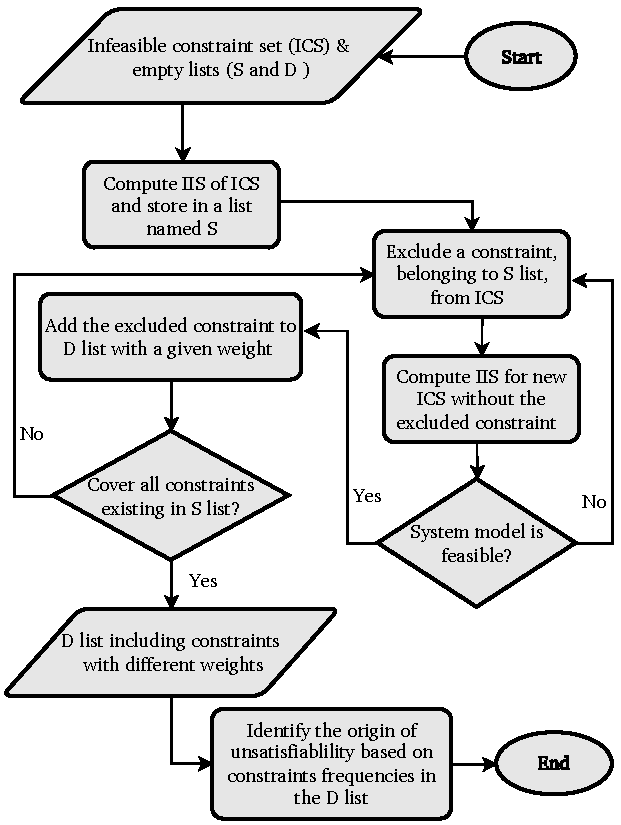
\includegraphics[width=0.7\columnwidth]{figures/flowchart_designerror.pdf}
    	\caption{The design error analysis flowchart using the IIS method.}
    	\label{fig61}
    \end{figure}
    
    
        %An algorithm is also introduced for this approach. Based on DVC algorithm, for each constraint of \textit{IIS\textunderscore list}, which is acquired from calculation of IIS for list of infeasible constraints or \textit{c\textunderscore list}, line number (1), it is excluded from the \textit{c\textunderscore list}, after finding the same constraint in the \textit{c\textunderscore list} (line number 2  to 5). Then, it is saved as the \textit{c\textunderscore list}. In other words, the \textit{c\textunderscore list} is updated (line number 5). The IIS is computed for the updated  \textit{c\textunderscore list} and stoted in \textit{result} (line number 6). If the result becomes null, the excluded constraint belonging to \textit{IIS\textunderscore list} or \textit{s} according to line (8), receives a weight and is saved in \textit{d\textunderscore list}. While, if \textit{s} constraint is already existed in the \textit{d\textunderscore list} (line 12), the assigned weight is added to its current weight (line 9 to 11 ).    
    
        Algorithm~\ref{DVC} is also introduced within this approach. Building upon the DVC algorithm, for each constraint present in the \textit{IIS\textunderscore list}, which is derived from the computation of IIS for the list of infeasible constraints, denoted as \textit{c\textunderscore list} (line number 1), it undergoes exclusion from the \textit{c\textunderscore list} upon encountering an identical constraint within it (lines 2 to 5). Subsequently, the modified constraint is saved back into the \textit{c\textunderscore list}, effectively updating it (line number 5).
        Following this, the IIS is recalculated for the updated \textit{c\textunderscore list} and stored within the \textit{result} variable (line number 6). If the result variable yields a null outcome, the constraint that was excluded, attributed either to the \textit{IIS\textunderscore list} or \textit{s} as per line (8), is assigned a weight and recorded within the \textit{d\textunderscore list}. However, in the scenario where the constraint \textit{s} already resides within the \textit{d\textunderscore list} (line 12), the assigned weight is incrementally added to its existing weight (lines 9 to 11).
        
        \subsubsection{ConstrIISForce}
        %When computing an IIS for an infeasible model, indicates whether the general constraint should be included or excluded from the IIS. The default value of $-1$ lets the IIS algorithm decide. If the attribute is set to $0$, the constraint is not eligible for inclusion in the IIS.If the attribute is set to $1$, the constraint is included in the IIS and the IIS algorithm never considers the possibility of removing it.
      %Note that setting this attribute to $0$ may make the resulting subsystem feasible (or consistent), which would then make it impossible to construct an IIS. Trying anyway will result in a GRB \textunderscore ERROR\textunderscore IIS\textunderscore NOT\textunderscore INFEASIBLE error. Similarly, setting this attribute to $1$ may result in an IIS that is not irreducible. More precisely, the system would only be irreducible with respect to the model elements that have force values of $-1$ or $0$.
    
        When determining an IIS for an infeasible model, the \textit{ConstrIISForce} parameter, as an attribute integrated into the Gurobi optimizer, determines the inclusion or exclusion of a general constraint within the IIS. If the value is set to $-1$ by default, the decision is left to the IIS algorithm itself. Alternatively, if the attribute is set to $0$, the constraint is deemed ineligible for the IIS inclusion. Conversely, setting the attribute to $1$ guarantees the constraint's inclusion in the IIS, with the algorithm disregarding any consideration of its removal~\cite{gurobi}.
        
      
        Note that configuring this attribute as $0$ can potentially make the derived subsystem feasible or consistent. Consequently, attempting to construct an IIS may lead to a GRB \textunderscore ERROR\textunderscore IIS\textunderscore NOT\textunderscore INFEASIBLE error, even if attempted. Similarly, assigning this attribute a value of $1$ may yield an IIS that lacks full irreducibility. The system's irreducibility pertains solely to model elements bearing force values of $-1$ or $0$~\cite{gurobi}. Hence, in order to remove a constraint in line (5) of the DVC algorithm, this parameter is utilized.  
    

    
    
    
        \begin{algorithm}[t]
        \SetAlgoLined
        \KwIn{A list of infeasible MIP constraints (\textit{c\textunderscore list}), $s$ $\in$ \textit{Constr}}
        \KwOut{Weighted constraints $S$}
        
            \textit{IIS}\textunderscore\textit{list} $\gets$ \textit{computeIIS(c\textunderscore list)};
            
             %\textit{Create an empty list (d\textunderscore list)};
             
        \For{$i\gets0$ \KwTo \textit{IIS}\textunderscore\textit{list}.\textit{size}}{
            
            \For{$j\gets0$ \KwTo \textit{c}\textunderscore\textit{list}.\textit{size}}{
            
            \If{ \textit{IIS}\textunderscore\textit{list.get(i) = c}\textunderscore\textit{list.get(j)}}{
            
            \textit{c\textunderscore list.remove(j)};
            
            \textit{result}$\gets$ \textit{c}\textunderscore\textit{list.computeIIS};
            
                \If{\textit{result == null}}{
                    
                     \textit{s}$\gets$\textit{IIS}\textunderscore\textit{list.get(i)};
                    
                    \eIf{\textit{s}$\in$ \textit{d\textunderscore list}}
                    {
                     %\State   
                     \textit{d\textunderscore list.get(s).setWeight(d\textunderscore list.get(s).get(Weight) $+$ 1)}; 
                        %$\gets$\textit{IIS}\textunderscore\textit{list.get(i)}
                        %\textit{s.get(Weight) $+$ setWeight(1)};
                    }
                    {\textit{d\textunderscore list.add(s.setWeight(1))};}
                    %\Else
                    %\State  
                    
                    %\If{\textit{s}$\notin$ \textit{d\textunderscore list}}{
                     %   \textit{d\textunderscore list.add(s.setWeight(1))};
                    %}
                 %\Else{\textit{s}$\notin$ \textit{d\textunderscore list}}
                 %\EndIf 
                    
                    }
            
                }
         }
        }
        \caption{DVC}
        \label{DVC}
        \end{algorithm}
    
 
    
    \subsection{Using MARCO Algorithm}
    
    %Another algorithm that will be utilized in this thesis is MARCO [Lif+16],which is a derivative of CAMUS[LS08b]. MARCO is used for enumerating MUSes (as well as MSSes) from unsatisfiable constraints as a SATproblem using hitting set dualization. The objective of MARCO is to explore the power set of the constraints P(C), given a set of constraintsC. I will first introduce the implementation of MARCO and then give an example of it by means of powerset lattice for visualization. MUS/MSS Duality any MCS of an instance is a minimal hitting set of the collection of MUSes for that instance, and any MUS is a minimal hitting set of the MCSes. The MARCO algorithm is following: As an additional supplement, the subroutines in the pseudocoodes are following: Grow(satisfiable subset X) RETURN MSS M One approach to finding an MSS is to start with a known-satisfiable subset X and "walk" up through the lattice by identifying SAT supersets. It’s important to note that this method is not equivalent to solving the Max-SAT problem, as an MSS may not have the largest possible cardinality
    
    %MARCO is an algorithm for analyzing infeasible constraint systems with the goal of enumerating all MUSes and maximal satisfiable subsets (MSSes). Typically, MUSes are of more interest, as they have found broader application~\cite{liffiton2016fast}.
     %MARCO is short for Mapping Regions of Constraints, and that roughly describes how it operates. This mapping can be represented visually on the power set lattice of a constraint system. The power set of a set of constraints is the set of all constraint subsets. 
        
    %In order to find the constraints that lead to unsatisfiability, a brute forcemethod can be used in which all the constraint’s frequencies in theMUS sets are counted and sorted by frequency~\cite{kleiman2009brute}. It is assumed that theconstraint with the highest frequency could be the one that leads tounsatisfiability. Changing this requirement will have a high chance ofmaking the constraint satisfiable. However, this method may not alwaysbe the most efficient as it can be computationally expensive, especiallyfor large systems with many constraints. 
        %To use the Marco algorithm, the introduced MIP constraints integrated in the \textit{E/E Designer} tool must be transformed to the SMT constraints. MIP constraints used in optimization problems involving both continuous and integer variables while SMT constraints utilized in logical constraint satisfaction problems involving complex logical formulas over various theories. After using the MARCO algorithm to generate all MUSes from the SMT constraints,the constraints are sorted and grouped according to their correspondingrequirements.
            %Then, the frequency of each constraint is analyzed toidentify the conditions that are most likely to cause the system to beunsatisfiable. This approach is similar to the IIS approach,where constraints were ordered based on their weights torecognize the most influential constraints. it should be added that after transforming the MIP to SMT constraints, Z3 solver is used to solve the set of SMT constraints~\cite{de2008z3}. In case of an infeasible solution, the generated SMT file by the Z3 solver is fused into the MARCO algorithm. In the last step, the frequency of each constraints is counted and the most critical constraints are investigated.
    
    MARCO is an algorithm designed to analyze infeasible constraint systems with the primary objective of systematically listing all MUSes and maximal satisfiable subsets (MSSes). Generally, MUSes hold a higher degree of significance due to their more comprehensive range of applications.
    MARCO is an acronym for Mapping Regions of Constraints, succinctly capturing its operational essence. The underlying concept revolves around mapping, which can be effectively visualized on the power set lattice of a given constraint system. The power set of constraints refers to the complete collection of all possible subsets of constraints within that set~\cite{liffiton2016fast}.
 
    
    To identify the constraints responsible for unsatisfiability, a brute-force method can be employed, involving the counting and sorting all constraints' frequencies in the MUS sets, as outlined in Kleiman et al.'s work~\cite{kleiman2009brute}. The constraint with the highest frequency may be the root cause of the unsatisfiability. Altering this criterion increases the likelihood of rendering the constraint satisfiable. However, this method may not always be the most efficient, as it can be computationally demanding, particularly for large systems encompassing numerous constraints.
    
    
 
    
    The MIP constraints introduced in the presented framework tool must be transformed into SMT constraints to use the MARCO algorithm. These type of constraints are used in optimization problems involving continuous and integer variables, while the SMT constraints are employed in logical constraint satisfaction problems with complex logical formulas across various theories.
    After employing the MARCO algorithm to generate all MUSes from the SMT constraints, the constraints are sorted and grouped based on their corresponding requirements.
    Next, the frequency of each constraint is analyzed to identify the conditions most likely to lead to system unsatisfiability. This approach shares similarities with the IIS approach, where constraints were prioritized based on their weights to identify the most influential ones. Following the transformation of the MIP to the SMT constraints, the Z3 solver is employed to solve the set of SMT constraints~\cite{de2008z3}. In cases of infeasible solutions after solving, the SMT file generated by the Z3 solver is integrated into the MARCO algorithm. In the final step, the frequency of each constraint is tallied, and the most critical constraints are investigated as the source of the unsatisfiability of the system model.
    
    Since the proposed framework includes the MIP constraints and utilizes the Gurobi optimizer, the IIS approach is preferred over the MARCO approach due to both the implementation effort involved and the effectiveness of the Gurobi solver in solving the MIP problems.
    
    
    %To implement the method for identifying core constraints in MARCOway, we divided the process into two main parts, as shown in Figure 5.3.The first part involves generating the constraint system, while the secondpart involves solving the model and extracting the core constraints fromthe MUSes.
    
    
    %In the constraint system generating part, we started by generating z3variables based on the input cores and applications. Then, we addedconstraints to the z3 model based on the requirements and output SMT2files. It’s worth noting that since MARCO is implemented in Pythonwhile our previous models were all in Java, we had to export the SMT2file from the model and then import it into MARCO.In the second part, we used MARCO to generate all the MUSes fromthe SMT constraints, and then counted the frequency of each constraintand grouped them by their corresponding requirements. Finally, wesorted the groups by frequency to identify the requirements that aremost likely to cause the system to be unsatisfiable, and thus the coreconstraints.
    
    %Power sets can be represented visually in Hasse diagrams, which provide a useful way to visualize all of the subsets and their relation to each other. In a Hasse diagram, every subset in the power set is represented by a node, and edges connect immediate supersets and subsets.
    
    
    
    
    
    
    
    
    
            
    %Another In order to find the requirements that lead to satisfiability\cite{liffiton2016fast}, a brute forcemethod can be used in which all the constraint’s frequencies in theMUS sets are counted and sorted by frequency. It is assumed that theconstraint with the highest frequency could be the one that leads tounsatisfiability. Changing this requirement will have a high chance of
    %making the constraint satisfiable. However, this method may not alwaysbe the most efficient as it can be computationally expensive, especiallyfor large systems with many constraints. Therefore, alternative methodsmay need to be explored to identify the most influential constraints moreefficiently.
    
    
    %\section{Implementation}
    
  
    
 
       \begin{figure}[ht]
    	\centering
    	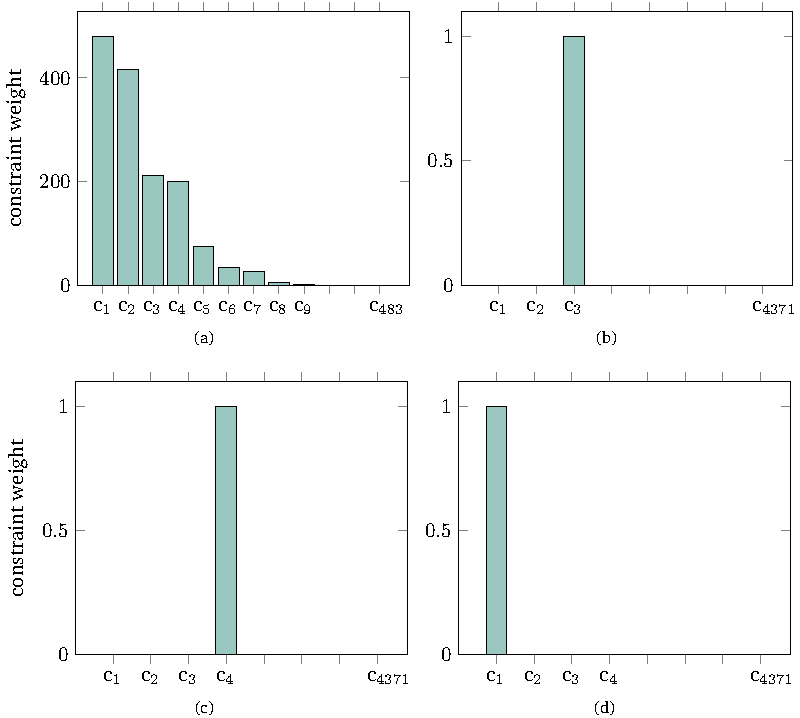
\includegraphics[width=0.98\columnwidth]{figures/designError_analysis.pdf}
    	\caption{The solutions of design error analysis approach created for various case studies using the IIS method.}
    	\label{fig62}
    \end{figure}
    \section{Evaluation}
    
    %In this section, the design error solutions generated by the introduced methods are provided and analyzed. For the IIS approach as the main design error analysis method used in the \textit{E/E Designer} tool, solutions for four different infeasible case studies are presented according to Fig.~\ref{fig62}. Fig.~\ref{fig62}~(a) depicts the weights of each constraint in an infeasible system model after solving including 15 ECUs, 6 applications, and 3 communication messages. The generated analysis shows that only eight constraints have a weight higher than zero out of 483 constraints. That being said that only eight constraints make the design model unsatisfiable. In addition, the higher weight of a constraint, the higher impact this constraint has on making the system model infeasible. 
    %For instance, in Fig.~\ref{fig62}~(a), the execution time of application threads were defined so close to their periods. As this error involve several constraints, different constraints were given weights based on their importance in causing an unsatisfiable model. In this example, c$_1$ has the highest weight which is related to the message routing constraints. Other constraints are relevant to the mapping and the time-triggered scheduling conditions. To correct the system model, the weighted constraints must be analyzed to find the source of violation. 
    
    This section provides and analyzes the design error solutions generated by the introduced methods. For the IIS approach, the primary design error analysis method used in the E/E Designer tool, solutions for four infeasible case studies are presented as shown in Figure~\ref{fig62}. Figure~\ref{fig62}~(a) depicts the weights of each constraint in an infeasible system model after solving, which includes 15 ECUs, six applications, and three communication messages. The generated analysis shows that only eight constraints have a weight higher than zero out of 483. This means that only these nine constraints render the design model unsatisfiable. Furthermore, the higher the weight of a constraint, the more significant its impact on making the system model infeasible.

     
    
    For instance, in Figure~\ref{fig62}~(a), the execution times of application threads were defined close to their respective periods. Since this error involves several constraints, different constraints were assigned weights based on their importance in causing an unsatisfiable model. In this example, c$_1$ has the highest weight related to the message routing constraints, while the other constraints are associated with the mapping and the time-triggered scheduling conditions. To correct the system model, the weighted constraints must be analyzed to identify the source of the violation.

      
    
    
    
 
    %In Fig.~\ref{fig62}~(b), the source of violation was identified for a modeled E/E system comprising 15 ECU, 60 applications, and 30 communication messages. In this model, the frame length of a communication message was specified higher than its period. As can be observed, only the constraint c$_3$, out of 4371 constraints, has a weight meaning that the condition, expressing the frame length of a message must be less than its period, became violated.
     %Since this violation does not involve the other conditions; hence, only the c$_3$ received a weight after the design error calculation using the IIS approach. In the next scenario, the same model as Fig.~\ref{fig62}~(b) is used. But, this time the execution time of an application thread is chosen higher than its period. So, as can be seen in Fig.~\ref{fig62}~(c) as the solution of the proposed approach using IIS, the related constraint c$_4$ received a weight out of other 4371 constraints; therefore, the user can get a feasible model after its solving by correcting the issue regarding this specific constraint. 
    In Figure~\ref{fig62}~(b), the source of violation was identified for a modeled E/E system comprising 15 ECUs, 60 applications, and 30 communication messages. In this model, the frame length of a communication message was specified to be greater than its period. As observed, only constraint c$_3$, out of 4371 constraints, has a weight, indicating that the condition stating that the frame length of a message must be less than its period was violated.
    Since this violation does not involve the other conditions, only c$_3$ received a weight after the design error calculation using the IIS approach. In the following scenario, the same model as in Figure~\ref{fig62}~(b) is used. However, this time, the execution time of an application thread is set higher than its period. As can be observed in Figure~\ref{fig62}~(c), which is the solution provided by the proposed approach using IIS, the related constraint c$_4$ received a weight from the other 4371 constraints. Therefore, the user can achieve a feasible model by correcting the issue related to this specific constraint during the solving process.
    
       \begin{figure}[b!]
    	\centering
    	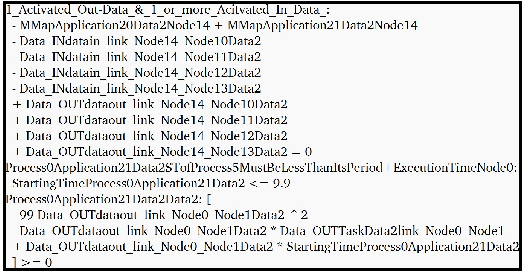
\includegraphics[width=1\columnwidth]{figures/iis_output1.pdf}
    	\caption{The partial output of IIS computation for the case study presented in figure~\ref{fig62}~(a).}
    	\label{fig63}
    \end{figure}
    %Finally, in Fig.~\ref{fig62}~(d), a routing constraint in the system model was changed which caused an infeasible model after solving step. This was done to check if the presented approach can find the exact source of violation. After applying the design error approach, the routing constraint or c$_1$ in fig.~\ref{fig62}~(d) was recognized.
       %Note that the computation time to find the source of unsatisfiability varies depending on if source of conflict impacts on a single constraint or multiple constraints. Also, it changes if the error is extremely obvious based on the defined constraints or if the error appears after solving the half of the system model due to adding the values to the model which makes the system infeasible. 
           %For example, in the use case of Fig.~\ref{fig62}~(a), the execution time of a thread was defined close to its period. This does not make any conflict at the first place based on the scheduling constraints. However, after finding the correct schedules for multiple applications, the overlapping between threads happened due to the small gap between their execution time and period which also causes conflicts on other conditions such routing. Therefore, the computation time plays pivotal role in extensive models particularly when the error involves multiple constraints.
      
    Finally, in Figure~\ref{fig62}~(d), a routing constraint in the system model was modified, resulting in an infeasible model after the solving step. This modification was done to verify whether the presented approach can accurately identify the source of the violation. Following the application of the design error approach, the routing constraint (c$_1$ in Figure~\ref{fig62}~(d)) was successfully identified.  

    Note that the computation time required to identify the source of unsatisfiability varies depending on whether the source of conflict impacts a single or multiple constraints. It also varies based on whether the error is self-explanatory, as defined by the constraints, or if the error becomes apparent only after solving half of the system model due to adding values that render the system infeasible.
    For example, in the use case shown in Figure~\ref{fig62}~(a), the execution time of a thread was defined to be close to its period. Initially, this does not appear to cause conflicts based on the scheduling constraints. However, after determining the correct schedules for multiple applications, it became evident that the overlapping between threads occurred due to the small gap between their execution time and period, leading to conflicts in other conditions, such as routing. Therefore, the computation time plays a pivotal role in extensive models, mainly when the error involves multiple constraints.
    
    
    
    
    %Fig.~\ref{fig63} shows partial output comprising 483 constraints after calculating the IIS for the infeasible model described in Fig.~\ref{fig62}~(a) using the \textit{computeIIS} command in the Gurobi optimizer. As can be observed, there are list of MIP constraints including their names. While, Fig.~\ref{fig64} shows the result of the designed error analysis approach for the presented case study in the Fig.~\ref{fig62}~(a). For each constraint name a weight has been calculated based on the Fig.~\ref{fig64}. 
    Figure~\ref{fig63} shows a partial output comprising 483 constraints after calculating the IIS for the infeasible model described in Figure~\ref{fig62}~(a) using the \textit{computeIIS} command in the Gurobi optimizer. As can be observed, a list of MIP constraints includes their names. Meanwhile, Figure~\ref{fig64} displays the results of the designed error analysis approach for the presented case study in Figure~\ref{fig62}~(a). A weight is calculated for each constraint name based on the information presented in Figure~\ref{fig64}.
        
        \begin{figure}[t]
    	\centering
    	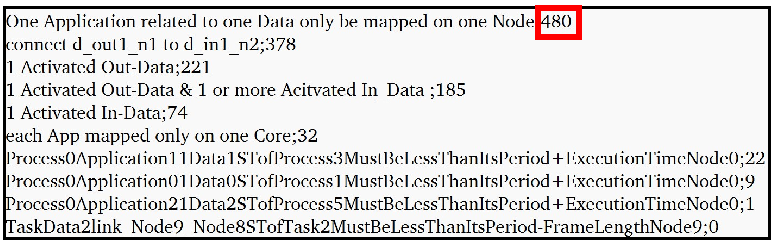
\includegraphics[width=1\columnwidth]{figures/de_output1.pdf}
    	\caption{The result of design error analysis approach using the IIS method for the use case described in figure~\ref{fig62}~(a).}
    	\label{fig64}
    \end{figure}
    %The solution consists of nine constraints with computed weights and the c$_1$ constraint has the highest influence, as the number in the red box indicates, on making the model infeasible as also explained in the Fig.~\ref{fig62}~(a). By this solution, the user can check the weighted constraints in order to correct the system to get a satisfiable solution after its solving.
        
    %An infeasible mapping case study was used to assess the design error analysis approach using the MARCO algorithm. This use case includes 16 ECUs and 13 applications. A similar result as the last described approach was acquired which comprised three constraints with given weights.
    
   The solution consists of nine constraints with computed weights, and the c$_1$ constraint has the highest influence, as indicated by the number in the red box, on making the model infeasible, as also explained in Figure~\ref{fig62}~(a). With this solution, the user can review the weighted constraints in order to correct the system and obtain a feasible solution after solving it.

    An infeasible mapping case study was conducted to assess the design error analysis approach using the MARCO algorithm. This use case involves 16 ECUs and 13 applications. Similar to the previously described approach, the results yielded three constraints with assigned weights. However, it is essential to acknowledge that the MARCO algorithm generates only one minimal unsatisfiable subset (MUS) based on specific constraints within the system. Consequently, the outcomes produced by the MARCO algorithm are significantly influenced by the precise number of constraints associated with particular requirements in the constraint system.
    To gain a more comprehensive insight into the infeasibility of the constraint system, it becomes imperative to execute the MARCO algorithm multiple times, each employing a distinct set of constraints.
 
    %\addtocounter{page}{1}
    %\newpage
    %\thispagestyle{empty}
        %\afterpage{\blankpage}
    
 

    
    
    
    %The presented solution exploits the power of logic programming to formulate adequate queries before schedule synthesis where the responses can be used to optimize the model and avoid e. g. bottlenecks. In this chapter, the focus is on situations where a designed network model is not satisfiable and no feasible schedules are found by the solver. In contrast to simple network models, localization and correcting unsatisfiability of complex network models is time-consuming and increases the development costs. To tackle this problem, a constraint labeling approach is presented which aims to assist the designers to better understand where in the model the unsatisfiability occurs i. e. there are conflicting constraints that cannot be satisfied at the same time. Only if the solving procedure terminates within acceptable time (depending on engineering requirements), network configuration or model correction can be started. To optimize the model before synthesis, Prolog-based queries are presented which aim at reducing the synthesis time by optimizing the network model. The presented solution exploits the power of logic programming to formulate adequate queries before schedule synthesis where the responses can be used to optimize the model and avoid e. g. bottlenecks.


  









